\chapter{电流及其效应}\label{ch:g8:electric-current-effects}

电流在五年的电路学习中默默地发挥着作用：
照亮灯丝、带动\omterm{ex:g6:circuits-and-safety:motor}{电动机}、发出蜂鸣声。
今年，电学转入定量研究——\omterm{def:g6:measurement-in-science:measuring}{测量}、\omterm{def:g6:measurement-in-science:measuring}{单位}与
定律。先来盘点一下：电流究竟能
\emph{做}什么？事实表明，电流有三种效应，
整个电学世界正是由它们构建而成。

\section{三种效应}

\begin{proposition}[电流的效应]\label{prop:g8:electric-current-effects:three}
电流通过物质时，会表现出三种效应：
\begin{enumerate}
  \item \emph{热效应}\index{热效应}：每一个电流都会使其经过的\omterm{def:g4:conductors-insulators:conductor}{导体}发热——
        良导线中温和地发热，
        细导线或过载的导线中则剧烈发热，
        而在灯丝和烤面包机中则被有意加热至白热；
  \item \emph{磁效应}\index{磁效应}：电流使其周围产生磁性——
        导线能使附近的\omterm{def:g4:magnets-and-compass:compass}{指南针}指针偏转，
        绕成线圈的导线则成为真正的\omterm{def:g1:magnets:magnet}{磁铁}，
        具有\omterm{def:g4:magnets-and-compass:poles}{磁极}，且可随意\omterm{ex:g3:first-electric-circuit:switch}{开关}；
  \item \emph{化学效应}\index{化学效应}：电流通过某些\omterm{def:g3:solids-liquids-gases:liquid}{液体}时，
        会引起化学变化——例如将水分解为两种\omterm{def:g3:solids-liquids-gases:gas}{气体}，
        给汤匙镀银，
        为每一节\omterm{def:g3:first-electric-circuit:battery}{电池}充电
        和放电。
\end{enumerate}
\end{proposition}

\begin{example}[热效应的应用]\label{ex:g8:electric-current-effects:heating}
有意为之的例子：烤面包机发光的加热丝、水壶中隐藏的线圈、
老式\omterm{def:g3:first-electric-circuit:bulb}{灯泡}白热的灯丝，以及被设计为先熔断的\omterm{def:g7:short-circuits-safety:fuse}{保险丝}。
不希望出现的情况：手机充电器发热、笔记本电脑底部发烫，
以及\omterm{def:g7:short-circuits-safety:device}{短路}的危害——你在前面学过，它是“坏人”的典型特征。
同一种效应，既是仆人，也是危险，
其强弱取决于电流的大小；这一“剂量”，我们将在下一章
学习如何\emph{\omterm{def:g6:measurement-in-science:measuring}{测量}}。
\end{example}

\begin{omfigure}
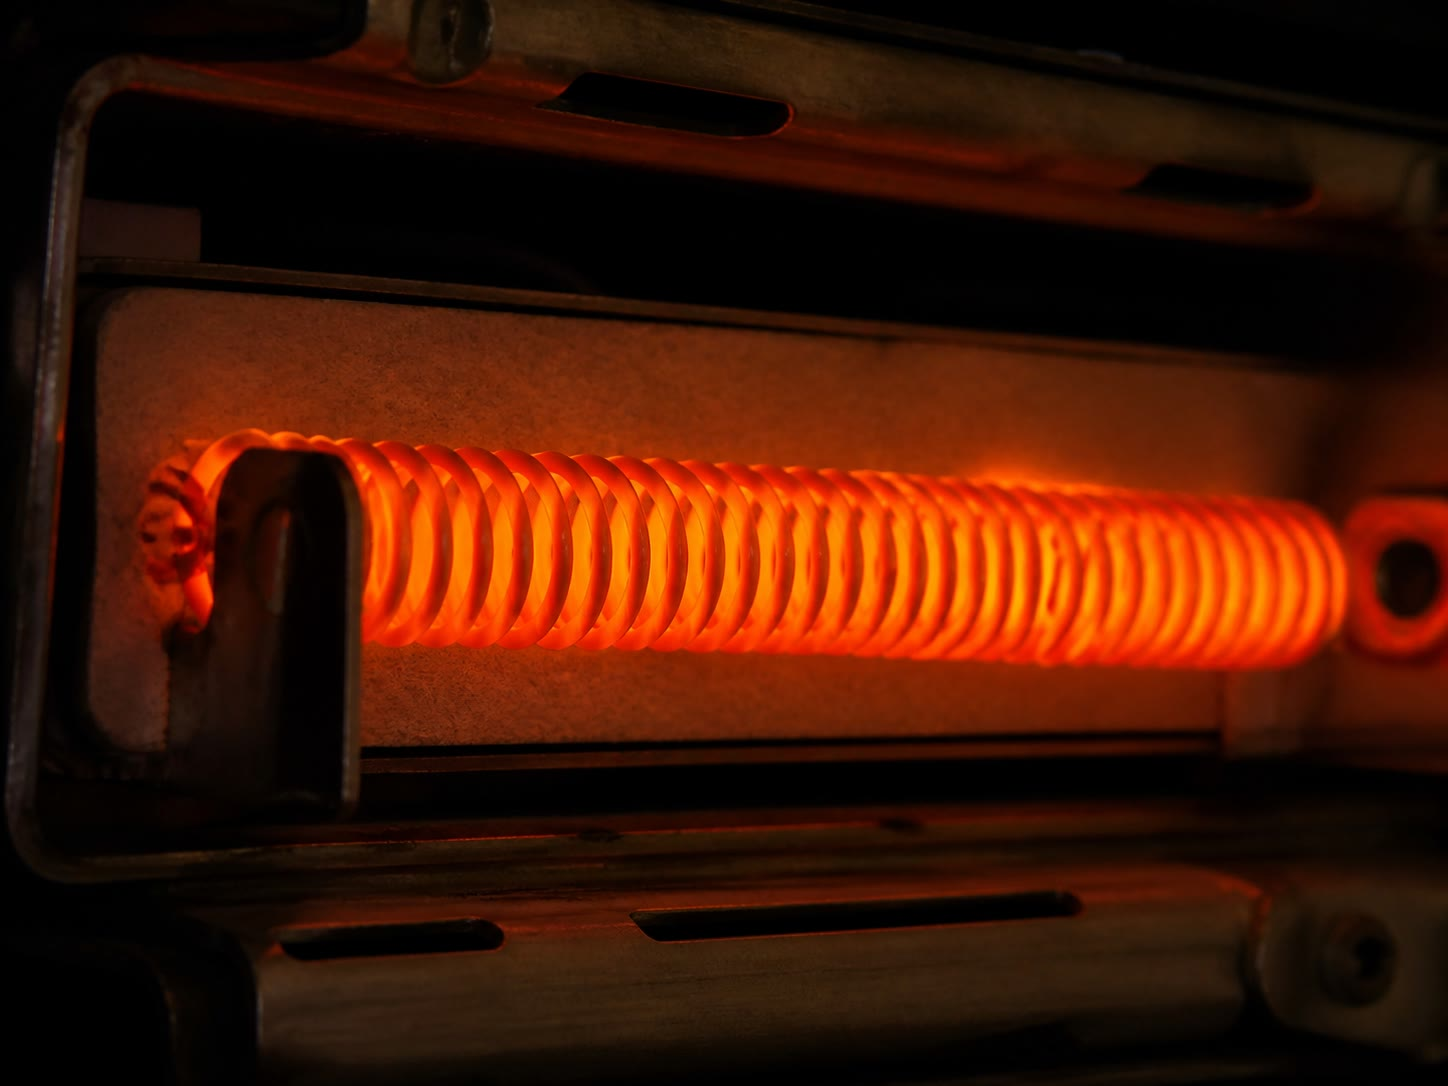
\includegraphics[width=0.5\linewidth]{images/book1/ai/g8-current-heating-coil.jpg}

{\small \omterm{prop:g8:electric-current-effects:three}{热效应}的发光现象：电流通过烤面包机的电阻丝，使其加热至炽红。}
\end{omfigure}

\section{电流产生磁性}

\begin{example}[指南针泄露了导线的秘密]\label{ex:g8:electric-current-effects:oersted}
两个世纪前，一位物理学家在讲课时注意到一件事：
每当他在旁边的实验台上接通电路，\omterm{def:g4:magnets-and-compass:compass}{指南针}指针都会微微抖动。
这种抖动——几乎只是指针的轻微颤动——
是人类首次看到电与磁之间的联系，
而在此之前，这两门学科就像天气与音乐一样毫不相干。
把\omterm{def:g4:magnets-and-compass:compass}{指南针}放在导线旁并接通电流：指针向一侧偏转；
将电流反向，指针则向另一侧偏转。
电流会在自身周围产生磁性，且磁性具有方向。
\end{example}

\begin{definition}[电磁铁]\label{def:g8:electric-current-effects:electromagnet}
\emph{电磁铁}\index{电磁铁}是由绝缘导线绕成的线圈，通常绕在铁芯上，
通电后即成为\omterm{def:g1:magnets:magnet}{磁铁}：具有\omterm{def:g4:magnets-and-compass:poles}{北极}和\omterm{def:g4:magnets-and-compass:poles}{南极}，
并能\omterm{def:g1:magnets:magnet}{吸引}铁质物体。与任何天然\omterm{def:g1:magnets:magnet}{磁铁}不同，它
受\omterm{ex:g3:first-electric-circuit:switch}{开关}控制：接通电流，磁性即有；
断开电流，磁性即消失；
反向通电，\omterm{def:g4:magnets-and-compass:poles}{磁极}随之对调。
\end{definition}

\begin{omfigure}
\begin{tikzpicture}[scale=0.85]
  \draw[thick, fill=omExo, fill opacity=0.3]
    (1.2,1.0) rectangle (5.4,1.9);
  \foreach \x in {1.5,2.1,...,5.1} {
    \draw[very thick, omDef] (\x,0.82) arc (200:340:0.35 and 0.5);
  }
  \draw[thick, omDef] (1.3,0.95) -- (0.4,0.4);
  \draw[thick, omDef] (5.3,0.95) -- (6.2,0.4);
  \node[below, font=\small] at (0.5,0.3) {接电池};
  \node[above, font=\small] at (3.3,2.05) {线圈中的铁芯};
  \draw[thick] (7.4,1.05) ellipse (0.32 and 0.14);
  \draw[thick] (8.15,1.3) ellipse (0.32 and 0.14);
  \draw[thick] (7.5,1.6) ellipse (0.32 and 0.14);
  \node[right, font=\small] at (8.7,1.3)
    {回形针：开关闭合时被吸住};
\end{tikzpicture}

{\small \omterm{def:g8:electric-current-effects:electromagnet}{电磁铁}：线圈与电流产生磁性，
\omterm{ex:g3:first-electric-circuit:switch}{开关}可使其产生、消失或翻转。}
\end{omfigure}

\begin{example}[可开关的磁性无处不在]\label{ex:g8:electric-current-effects:uses}
废料场中的起重机用\omterm{def:g8:electric-current-effects:electromagnet}{电磁铁}吸起汽车，
再断开\omterm{ex:g3:first-electric-circuit:switch}{开关}将其放下——用天然\omterm{def:g1:magnets:magnet}{磁铁}可做不到。
电动门锁、继电器的咔嗒声、门铃的锤子
（\omterm{def:g8:electric-current-effects:electromagnet}{电磁铁}将锤子吸向铃身，切断自身电流后又弹回：
这种“嗒嗒”声就是磁性的规律体现）、老式电话的听筒，
以及最重要的——每一台\omterm{ex:g6:circuits-and-safety:motor}{电动机}：电流产生的磁性
与\omterm{def:g1:magnets:magnet}{磁铁}相互推斥，每秒可达成千上万次。
\omterm{prop:g8:electric-current-effects:three}{磁效应}是
电气时代的“肌肉”。
\end{example}

\begin{method}[绕制电磁铁]\label{met:g8:electric-current-effects:wind}
\begin{enumerate}
  \item 将一到两米长的细绝缘导线紧密、整齐地
        绕在一根大铁钉或螺栓上，
        留出两个自由端；
  \item 通过\omterm{ex:g3:first-electric-circuit:switch}{开关}将两端接到\omterm{def:g3:first-electric-circuit:battery}{电池}上（不要长时间直接相接——
        线圈几乎相当于\omterm{def:g7:short-circuits-safety:device}{短路}，会发热：
        \omterm{prop:g8:electric-current-effects:three}{热效应}在此实验中起到了“护航”的作用
        ）；
  \item 短暂闭合\omterm{ex:g3:first-electric-circuit:switch}{开关}：钉帽吸起回形针；
        断开\omterm{ex:g3:first-electric-circuit:switch}{开关}：回形针落下；
  \item 用\omterm{def:g4:magnets-and-compass:compass}{指南针}检验：线圈两端表现为 N 极和
        S 极——\omterm{def:g3:first-electric-circuit:battery}{电池}反接时两者对调。
\end{enumerate}
匝数越多，吸力越强：通过绕线调节磁性的“剂量”。
\end{method}

\section{化学效应}

\begin{example}[水中的电流]\label{ex:g8:electric-current-effects:electrolysis}
将两根与\omterm{def:g3:first-electric-circuit:battery}{电池}相连的铅笔芯电极浸入
稍微导电的水中（加一小勺洗衣碱会有帮助），然后
观察：两根电极都冒出细小气泡——两种不同的
\omterm{def:g3:solids-liquids-gases:gas}{气体}，都由水本身生成，其中一根电极处产生的
\omterm{def:g6:mass-and-volume:volume}{体积}是另一根的两倍。电流正把水拆解为
两种看不见的组分。电与化学之间的这扇门——
\emph{电解}——为廉价的勺子镀上
银、从矿石中提炼铝，它主要属于你的
化学课程；物理学只向它致意，便继续前行。
\end{example}

\begin{example}[每块电池都是化学效应的逆过程]\label{ex:g8:electric-current-effects:battery}
在每块\omterm{def:g3:first-electric-circuit:battery}{电池}内部，化学作用推动着电流：储存的
化学能驱动这股电流，在为电路服务的同时逐渐耗尽
——你自手电筒变暗那天起就熟悉的耗尽过程。
可充电\omterm{def:g3:first-electric-circuit:battery}{电池}闭合了这一循环：充电器迫使电流
\emph{反向}通过，\omterm{prop:g8:electric-current-effects:three}{化学效应}重新
储存\omterm{def:g5:everyday-energy:energy}{能量}。化学能转为电能，电能转为化学能：
一种效应、两个方向，撑起整个\omterm{def:g3:first-electric-circuit:battery}{电池}产业。
\end{example}

\begin{remark}[作为探测器的效应]\label{rem:g8:electric-current-effects:detect}
三种效应回答了一个曾经难倒你的问题——当测试员学徒时，
你就已经想问：如何\emph{看见}一股电流——
不透明导线中那股看不见的“行进”？靠它的作用来看。升温的
导线、颤动的\omterm{def:g4:magnets-and-compass:compass}{指南针}、冒出的气泡：每一种都暴露了
这股行进。迄今制成的每种测电流仪器，都读取
三种效应之一——而下一章中等待我们的那种仪器
读取的是\omterm{prop:g8:electric-current-effects:three}{磁效应}的颤动，并被细化为带刻度的
表盘。
\end{remark}

\section{练习}

\begin{exercise}[$\star$]\label{exo:g8:electric-current-effects:1}
说出电流的三种效应，并各举一例其
服务于人的用途。
\end{exercise}

\begin{exercise}[$\star$]\label{exo:g8:electric-current-effects:2}
判断下列各场景分别对应哪种效应：\omterm{def:g7:short-circuits-safety:fuse}{保险丝}熔断；\ 门铃
敲击；\ 铅笔芯处冒出的气泡；\ 烤面包机的发光；
\ 废料场起重机的吸力？
\end{exercise}

\begin{exercise}[$\star$]\label{exo:g8:electric-current-effects:3}
讲台旁颤动的\omterm{def:g4:magnets-and-compass:compass}{指南针}揭示了什么？
电流反向时，这种颤动会发生什么变化？
\end{exercise}

\begin{exercise}[$\star$]\label{exo:g8:electric-current-effects:4}
列举\omterm{def:g8:electric-current-effects:electromagnet}{电磁铁}具有、而天然磁石无法比拟的三种
能力。
\end{exercise}

\begin{exercise}[$\star$]\label{exo:g8:electric-current-effects:5}
在绕线法中，导线为何必须绝缘？还有，
为何线圈不能在未接用电器\omterm{def:g2:measuring-time:duration}{时长}时间保持接通？
\end{exercise}

\begin{exercise}[$\star$]\label{exo:g8:electric-current-effects:6}
起重机操作员如何松开吊起的废车？请与
同等强度天然磁石所需的做法相比较。
\end{exercise}

\begin{exercise}[$\star$]\label{exo:g8:electric-current-effects:7}
\omterm{def:g3:first-electric-circuit:battery}{电池}使用时内部发生了怎样的\omterm{def:g5:everyday-energy:energy}{能量}转化？还有，
可充电\omterm{def:g3:first-electric-circuit:battery}{电池}在充电器上时，内部又如何？
\end{exercise}

\begin{exercise}[$\star$]\label{exo:g8:electric-current-effects:8}
三种效应作为\emph{探测器}，为何如此宝贵？哪一种
效应将在下一章的仪器中被细化为
一个数值？
\end{exercise}

\begin{exercise}[$\star\star$]\label{exo:g8:electric-current-effects:9}
门铃：\omterm{def:g8:electric-current-effects:electromagnet}{电磁铁}将锤子猛拉向铃，
但运动中的锤子会断开自身的电路；弹簧
将锤子弹回，重新接触，如此往复。请走完
一个完整周期，并解释该设计为何\emph{必须}
持续作响，而非保持吸合。
\end{exercise}

\begin{exercise}[$\star\star$]\label{exo:g8:electric-current-effects:10}
继电器是由\omterm{def:g8:electric-current-effects:electromagnet}{电磁铁}闭合的\omterm{ex:g3:first-electric-circuit:switch}{开关}：线圈中的小电流
闭合那些在另一电路中承载大电流的触点。
试解释为何这一方式能让灵敏的恒温器安全地
操控耗电的电暖器——并指出哪两个电路
从不相接。
\end{exercise}

\begin{exercise}[$\star\star$]\label{exo:g8:electric-current-effects:11}
只要墙内隐藏的导线中有电流通过，你的\omterm{def:g4:magnets-and-compass:compass}{指南针}
指针就会颤动。据此设计一个墙内导线探测器：
写出操作步骤、强烈颤动所代表的含义，以及该仪器的
一项局限（想一想还有什么东西会使\omterm{def:g4:magnets-and-compass:compass}{指南针}转动）。
\end{exercise}

\begin{exercise}[$\star\star\star$]\label{exo:g8:electric-current-effects:12}
简述\omterm{ex:g6:circuits-and-safety:motor}{电动机}的原理：绕在轴上的线圈置于
\omterm{def:g1:magnets:magnet}{磁铁}的两极之间；电流使线圈成为磁体；
\omterm{def:g4:magnets-and-compass:poles}{磁极}间的推拉作用使轴转动——就在线圈
即将稳定地与磁场对齐时，流经它的电流被反向，因此它
必须永远追逐对齐。请逐极解释，为何
电流反向不可或缺——若没有它，\omterm{ex:g6:circuits-and-safety:motor}{电动机}会怎样？
（你刚刚解释了为何\omterm{ex:g6:circuits-and-safety:motor}{电动机}含有换向
触点——这也揭示了电气时代让车轮转动的
另一半原理）。
\end{exercise}

\section{问题：发明家的工坊}

\begin{problem}[{周末问题——一节电池、三种效应、
五项发明；发明家工坊里的
一个夜晚}]\label{pb:g8:electric-current-effects:1}
工作台上放着\omterm{def:g3:first-electric-circuit:battery}{电池}、导线、铁钉、
一只\omterm{def:g4:magnets-and-compass:compass}{指南针}、两根铅笔芯、一罐苏打水——
以及一本记满半成品发明、等待评估的笔记本。

\medskip\noindent\textbf{第一部分——清点器材。}
\begin{enumerate}
  \item 画出工坊的三效应试验台：
        对于一节\omterm{def:g3:first-electric-circuit:battery}{电池}和一个\omterm{ex:g3:first-electric-circuit:switch}{开关}，描述一种装置，能同时展示
        三种效应（细导线用来发热，\omterm{def:g4:magnets-and-compass:compass}{指南针}
        放在铅笔芯旁，罐子接入回路中）。三个演示应采用
        何种连接方式——
        \omterm{def:g4:series-circuits:series}{串联}还是\omterm{def:g5:series-parallel-circuits:parallel}{并联}，才能让一个\omterm{ex:g3:first-electric-circuit:switch}{开关}同时接通三者？
  \item 细演示导线发热，而粗供电导线
        仍保持凉爽，二者处于同一回路中。哪一条
        第一章关于\omterm{def:g4:series-circuits:series}{串联}回路的知识使此现象
        比看上去\emph{更}有意思——两根导线中什么量相等，
        什么量不同？
  \item \omterm{ex:g3:first-electric-circuit:switch}{开关}闭合时，\omterm{def:g4:magnets-and-compass:compass}{指南针}向东偏转。同时作出的
        哪两项改动，会使偏转
        与原来完全一样？
  \item 一根铅笔芯冒出的气泡\omterm{def:g7:motion-average-speed:formula}{速度}
        恰为另一根的两倍。这提示了水的两种
        组成成分有何端倪？（化学课将证实这一比例。）
\end{enumerate}

\medskip\noindent\textbf{第二部分——评估各项发明。}
\begin{enumerate}[resume]
  \item 发明：“无声门铃”——一个\omterm{def:g8:electric-current-effects:electromagnet}{电磁铁}，
        一次吸动柔软的毡制锤子，并将其吸住，
        直到按钮松开。经典门铃机构中，发明者必须
        \emph{去掉}哪个部件，
        访客会听到什么？
  \item 发明：“磁力分拣机”——传送带上的废料
        经过一个\omterm{def:g8:electric-current-effects:electromagnet}{电磁铁}下方，它吸起
        铁和钢。落料箱处会发生什么，为何
        分拣机会让铝罐留在传送带上
        （以往学过的两条磁学知识可作答）？
  \item 发明：“\omterm{def:g4:magnets-and-compass:poles}{磁极}翻转器”——一只\omterm{def:g4:magnets-and-compass:compass}{指南针}安装在
        线圈上方，每当一个隐藏\omterm{ex:g3:first-electric-circuit:switch}{开关}
        将\omterm{def:g3:first-electric-circuit:battery}{电池}反接时\omterm{def:g4:magnets-and-compass:compass}{指南针}便翻转。这是利用了
        电流磁性的哪一性质？
  \item 发明：“永动电镀机”——银电镀，
        由一节“能从镀层中自行充电”的\omterm{def:g3:first-electric-circuit:battery}{电池}供电，
        请否决此设计，援引本章的两种\omterm{def:g3:first-electric-circuit:battery}{电池}接入方向
        及一条较早学过的\omterm{def:g5:everyday-energy:energy}{能量}守恒定律。
\end{enumerate}

\medskip\noindent\textbf{第三部分——夜晚的杰作。}
发明家以一个游园会上的抓物机收尾：一个操纵杆，
一个用细绳悬挂的小\omterm{def:g8:electric-current-effects:electromagnet}{电磁铁}，一箱铁制小玩意儿。
\begin{enumerate}[resume]
  \item 用效应的语言写出制胜一步的过程：
        在“抓取”时、摆动过程中以及
        “释放”时分别发生什么？
  \item 游客抱怨抓物机在摆动中途掉落奖品，
        每当旧\omterm{def:g3:first-electric-circuit:battery}{电池}电量下降时。\omterm{def:g8:electric-current-effects:electromagnet}{电磁铁}的哪一性质
        ——一身兼具优点与弱点——
        正在此显现？
  \item 发明家将线圈匝数加倍以求改善。预测
        对抓取的影响，并说出另一个“剂量”
        （来自\omterm{def:g3:first-electric-circuit:battery}{电池}一侧），下一章将使我们能为其定量。
  \item 笔记本的最后一页：写下工坊的总结——
        每种效应各写一句，各自点名它今晚最得力的
        发明。
\end{enumerate}
\end{problem}
